\section{Théorie}

\begin{minipage}{\linewidth}
    \begin{wrapfigure}{hR}{0.4\textwidth}
        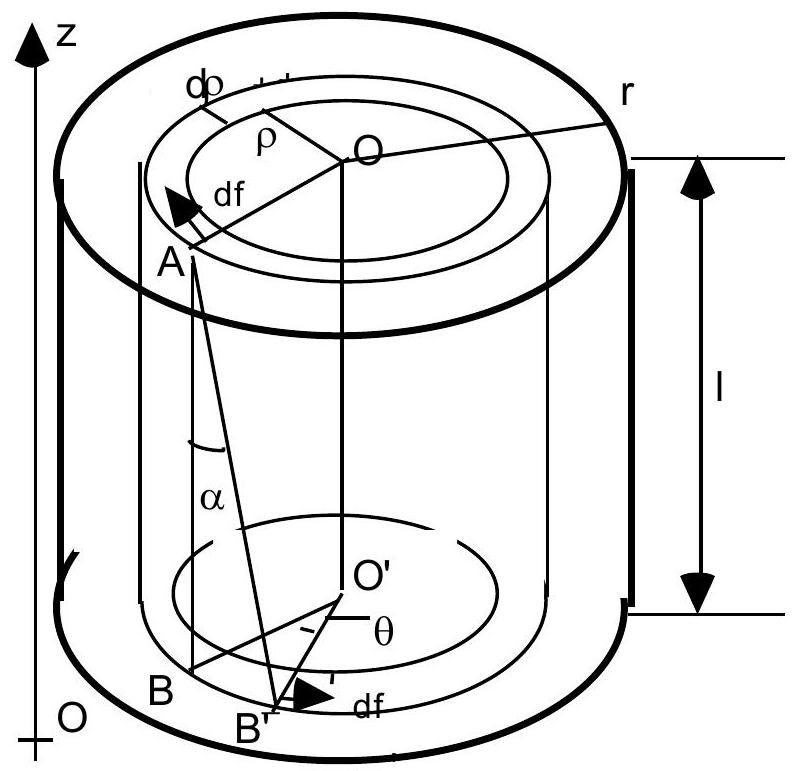
\includegraphics[width=0.35\textwidth]{figures/torsion.png}
        \caption{Schéma de la torsion d'un cylindre \cite{notice}}
        \label{fig:torsion}
    \end{wrapfigure}
    
    Le sujet d'intérêt des expériences présentées ici était principalement le module de cisaillement $G$ des matériaux étudiés. Il est défini par $\tau = G\alpha$ avec $\tau$ la contrainte de cisaillement et $\alpha$ l'angle de déformation. Dans le cas d'un cylindre tordu par une rotation autour de son axe il est possible d'obtenir:
    \begin{equation}
        \alpha \approx \tan(\alpha) \approx \frac{\rho \theta}{l}
    \end{equation}
    avec $\rho$ la distance au centre du cylindre, $\theta$ l'angle de déplacement par rapport à l'axe principal et $l$ la longueur du cylindre comme illustré dans la \autoref{fig:torsion}. Cela permet d'obtenir une expression pour le moment des forces:
    \begin{equation}
        M(\theta) = \int_{S}\rho\tau dS = \int_{0}^{r}2\pi\rho G \frac{\rho \theta}{l} \rho d\rho = \frac{\pi G\theta d^4}{32l}
    \end{equation}
    Dans le cas de la méthode statique qui consiste à appliquer un moment de forces en attachant un poids à un disque de diamètre $D$ cela donne donc:
    \begin{equation}
        \frac{\pi G\theta d^4}{32l} = mg\frac{D}{2} \Rightarrow G = \frac{16 l m g D}{\pi d^4 \theta}
        \label{eq:module_cisaillement_statique}
    \end{equation}
\end{minipage}

Pour la méthode dynamique, l'équation du mouvement est $I\ddot{\theta} + M(\theta) = 0$ ce qui donne $\theta = \theta_0\cos(\omega t+ \varphi)$ avec:
\begin{equation}
    \omega = \sqrt{\frac{\pi G d^4}{32 l I}}
\end{equation}
Ce qui donne sachant l'expression de la période $T = \frac{2\pi}{\omega}$:
\begin{equation}
    G = \frac{128 \pi I l}{d^4 T^2}
    \label{eq:module_cisaillement_dynamique}
\end{equation}

En réalité il s'agit plutôt d'un oscillateur amorti avec donc une décroissance donnée par cette nouvelle solution:
\begin{equation}
    \theta(t) = \theta_0 \exp(-\lambda t) \cos(\omega t + \varphi)
\end{equation}
où $\lambda$ est le coefficient d'amortissement du matériau.
Avec la valeur de la période $T$ et $n \in \mathbb{N}$ il est possible d'écrire:
\begin{equation}
    \cos(\omega t + \varphi) = \cos(\omega (t + nT) + \varphi) = C(t)
    \label{eq:cos_equal}
\end{equation}
ce qui donne:
\begin{equation}
    \theta_0 = \frac{\theta(t) e^{\lambda t}}{C(t)}
    \quad \Rightarrow \quad
    \theta(t+nT) = \theta(t)e^{\lambda(t - t - nT)} \frac{C(t)}{C(t)}
\end{equation}
en utilisant toujours l'\autoref{eq:cos_equal}. Cela permet finalement d'obtenir:
\begin{equation}
    \ln\left(\frac{\theta(t+nT)}{\theta(t)}\right) = -\lambda nT , \quad
    \lambda = \frac{1}{nT} \ln \frac{\theta(t)}{\theta(t+nT)}
    \label{eq:decrement_log}
\end{equation}
